\documentclass{article}
\usepackage{mainPoly}

\title{Ensembles de nombres : arithmétique, intervalle}
\date{}
\author{Seconde 9}

\begin{document}
\maketitle

\section{Introduction}
\begin{tcolorbox}
\begin{definition}
Un \textbf{ensemble de nombres} est une collection de nombres partageant la même nature.
\end{definition}
\end{tcolorbox}
\begin{example}
On peut parler de l'ensemble des nombres renvoyés par un dé, ou l'ensemble des âges des élèves de la classe de seconde 9, ou encore l'ensemble de tous les prix affichés dans un supermarché.
\end{example}
\textbf{Par la suite, nous allons nous intéresser à différents ensembles classiques de nombres, et voir la façon dont sont étudiés les nombres associés.}
\section{Nombres entiers}
\subsection{Ensembles}
\begin{definition}
\hfill
\begin{itemize}
\item On note $\N$ l'ensemble des nombres entiers \textbf{Naturels} : il s'agit de tous les entiers plus grands ou égaux à $0$, comme $0$; $1$; $2$ \dots
\item On note $\Z$ l'ensemble des nombres entiers \textbf{relatifs} : il s'agit des entiers supérieurs, inférieurs ou égaux à \textbf{Zéro}, comme $-2$; $-1$; $0$; $1$; $2$ \dots
\end{itemize}
\end{definition}
\begin{definition}
\hfill

Pour dire qu'un nombre $n$ est un entier naturel, on écrit $n \in \N$. Cela se lit \emph{\og $n$ appartient à $\N$ \fg}.

Pour dire qu'un nombre $n$ est un entier relatif, on écrit $n \in \Z$. Cela se lit \emph{\og $n$ appartient à $\Z$ \fg}.
\end{definition}
\begin{example}
Vrai ou faux ? Répondre dans chacun des cas suivants.
\begin{enumquestions}
\begin{minipage}{0.45\textwidth}
\item $6 \in \N$ \answersline
\item $-9 \in \N$ \answersline
\item $-4 \in \Z$ \answersline
\end{minipage}
\hfill
\begin{minipage}{0.45\textwidth}
\item $12 \in \Z$ \answersline        
\item $5 \notin \N$ \answersline
\item $-8 \notin \N$ \answersline
\end{minipage}
\end{enumquestions}
\end{example}
\begin{proposition}
Tout nombre entier naturel est un nombre entier relatif. Du point des ensembles, cette proposition se note $\N \subset \Z$.
\end{proposition}
\begin{example}
Placer les nombres suivants dans le schéma : $5$; $2$; $-10$; $0$ et $-6$.
\begin{center}
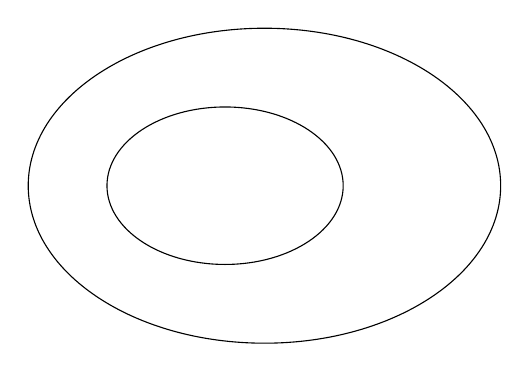
\begin{tikzpicture}
\draw (0,0) ellipse (3 and 2);
\draw (-0.5,0) ellipse (1.5 and 1);
\draw (2.5,0) node {$\Z$};
\draw (0.5,0) node {$\N$};
\end{tikzpicture}
\end{center}
\end{example}
\newpage
\subsection{Arithmétique}
\textbf{Nous travaillons avec les nombres de $\Z$. Dans ce contexte, on ne considère pas les divisions réelles, ni les fractions.}
\begin{tcolorbox}
\begin{definition}
Soit $a$ et $b$ deux entiers relatifs.
\begin{itemize}
\item $a$ est un \textbf{multiple} de $b$ si et seulement si il existe $k \in \Z$ tel que $a = k \times b$.
\item $b$ est un \textbf{diviseur} de $a$ si et seulement si il existe $k \in \Z$ tel que $a = k \times b$.
\end{itemize}
\end{definition}
\end{tcolorbox}
\begin{example}
\hfill
\begin{itemize}
\item Le nombre $10$ est un multiple de $2$ : en effet, il existe un nombre entier relatif $k = 5$ tel que $10 = k \times 2$.
\item Le nombre $7$ est un diviseur de $-28$ : en effet, il existe un nombre entier relatif $k = -4$ tel que $28 = k \times 7$.
\end{itemize}
\end{example}
\begin{example}
\hfill

Le nombre $36$ est-il un multiple de $3$ ? Justifier. \answersline

Le nombre $-8$ est-il un diviseur de $128$ ? Justifier. \answersline
\end{example}

\begin{remark}
Tout nombre est divisible par $0$. Ou, de façon équivalente, $0$ est le multiple de n'importe quel nombre. 
\end{remark}

\begin{proposition}
La somme de deux multiples de $a$ est un multiple de $a$.
\end{proposition}
\begin{proof}
\hfill
\vspace*{0.5cm}
\hfill
\emptybox{7cm}
\end{proof}
\newpage
\begin{definition}
\hfill
\begin{itemize}
\item Un nombre entier relatif est \textbf{pair} si et seulement s'il est divisible par $2$.
\item Un nombre entier relatif est \textbf{impair} si et seulement s'il n'est pas pair. 
\end{itemize}
\end{definition}
\begin{example}
\hfill

Le nombre $12$ est pair : en effet, il est divisible par $2$, car $12 = 2 \times 6$.

Le nombre $-27$ est impair : en effet, il n'est pas pair, car il n'existe pas d'entier relatif $k$ vérifiant $-27 = 2 \times k$.
\end{example}

\begin{proposition}
Un nombre $n \in \Z$ est impair si et seulement si il existe $p \in \Z$ tel que $n = 2 \times p + 1$.
\end{proposition}

\begin{proposition}
Soit $x$ et $y$ deux entiers relatifs. Alors, les tableaux suivants décrivent la parité de $x + y$ et de $x \times y$.
\vspace*{0.5cm}

\begin{minipage}{0.30\textwidth}
\begin{tabular}{|c|c|c|}
\hline
$x + y$&$y$ pair&$y$ impair\\
\hline
$x$ pair&pair& impair\\
\hline
$x$ impair& impair& pair\\
\hline
\end{tabular}    
\end{minipage}
\hfill
\begin{minipage}{0.30\textwidth}
\begin{tabular}{|c|c|c|}
\hline
$x \times y$&$y$ pair&$y$ impair\\
\hline
$x$ pair&pair& pair\\
\hline
$x$ impair& pair& impair\\
\hline
\end{tabular}    
\end{minipage}
\hfill
\begin{minipage}{0.30\textwidth}
\begin{tabular}{|c|c|c|}
\hline
$x^2$&$x$ pair&$x$ impair\\
\hline
&pair& impair\\
\hline
\end{tabular}    
\end{minipage}
\end{proposition}
\begin{proof}
On démontre ici uniquement la propriété suivante : si $x$ est un entier relatif impair, alors $x^2$ est impair.
\vspace*{0.5cm}

\emptybox{7cm}
\end{proof}

\newpage
\begin{tcolorbox}
\begin{definition}
Un nombre entier naturel $n \in \N$ est \textbf{premier} si et seulement si il admet exactement deux diviseurs positifs : $1$ et lui-même. 
\end{definition}
\end{tcolorbox}
\begin{remark}
\hfill
\begin{itemize}
\item Traditionnellement, un nombre premier est \textbf{positif} : on ne s'intéresse qu'aux entiers naturels dans ce cadre.
\item Le nombre $1$ n'est \textbf{\textsc{pas}} premier : il n'admet qu'un seul diviseur positif. 
\end{itemize}
\end{remark}
\begin{example}
Les nombres suivants sont premiers: $2; 3; 5; 7; 11; 13; 17; 19 \dots$
\end{example}
\begin{proposition}
Tout entier naturel supérieur ou égal à $2$ peut s'écrire comme un produit de nombres premiers. 
\end{proposition}
\begin{example}
\hfill
\begin{itemize}
\item $18 = 2 \times 3 \times 3$
\item $68 =$ \answersline 
\item $132 =$ \answersline
\item $85 =$ \answersline
\end{itemize}
\end{example}
\begin{example}
On peut écrire des fractions sous forme irréductible à l'aide de la décomposition du numérateur et du dénominateur en produit de facteurs premiers.
\begin{itemize}
\item $\dfrac{500}{75} = \dfrac{2 \times 2 \times 5 \times \cancel{5} \times \cancel{5}}{3 \times \cancel{5} \times \cancel{5}} = \dfrac{2 \times 2 \times 5}{3} = \dfrac{20}{3}$
\item $\dfrac{126}{24} =$ \answersline
\item $\dfrac{3}{45} =$ \answersline
\end{itemize}
\end{example}

\end{document}

